\documentclass[a4paper,titlepage,10pt]{article}

\usepackage[margin=0.6in]{geometry} % margenes
\usepackage[spanish]{babel} % Le indicamos a LaTeX que vamos a escribir en español.
\usepackage[utf8]{inputenc} % Quiero acentos
\usepackage{caratula}
\usepackage{verbatim} % Para hacer código
\usepackage{graphicx} % Graficos
\usepackage[space]{grffile} % Espacios en el nombre de archivo de includeGraphics
\usepackage{multicol} % Multicolumna

\titulo{Super Collider}
\fecha{23 / 10 / 2013}
\materia{Teoría de Lenguajes}
\grupo{Grupo 12}
\integrante{Carreiro, Martin}{45/10}{martin301290@gmail.com}
\integrante{Kujawski, Kevin}{459/10}{kevinkuja@gmail.com}
\integrante{Ortiz De Zarate, Juan Manuel}{403/10}{jmanuoz@gmail.com}

\begin{document} % Todo lo que escribamos a partir de aca va a aparecer en el documento.

\maketitle

\section{Gramática}
Presentamos la siguiente gramática para el lenguaje dado:

$G_{sc} = (V_t,V_n,Prod,S)$\\

A continuación, se indica el significado de cada una de las variables mencionadas en la gramática: \\

$V_t$ = \{; , . , { , } , con , \& , mix , + , add , - , sub , * , mul , / , div , sin , ( , 
	lin , sil , noi , noise , sin , ) , play , post , loop , tune , fill , reduce , expand,
	0 , 1 , 2 , 3 , 4 , 5 , 6 , 7 , 8 , 9 , 0 , $\lambda$\}\\

$V_n$ = \{S , O , G , P , N , M , R , E , Z , Q\}\\

Siendo $Prod$:

\begin{verbatim}
S -> G | S.P | SOS | {S}
O -> ; | con | & | mix | + | add | - | sub | * | mul | / | div
G -> sin(N,R) | lin(R,R) | silQ | noi(R) | R | noise | sin(N)
P -> play(R) | postQ | loop(N) | tune (E) | fill(R) | reduceQ | expandQ | playQ
N -> 0|..|9|0N|1N|..|9N
M -> ZN.N
R -> N | M | E
E -> +N | -N 
Z -> + | - | \lambda
Q -> () | \lambda
\end{verbatim}

Descripcion:
Basicamente la gramatica se puede dividir en tres categorias cuyo resultando siempre seran buffers: Generadores, Metodos (con parentesis opcionales si no tienen parametros) y Numeros, que estos ultimos a su vez se dividen en enteros, naturales y racionales, para que cada metodo reciba el tipo de parametro que le corresponde. Además, adaptamos la gramatica para que permita los ejemplos del enunciado que no cumplen las formas de escritura por considerarlos como abrevaciones o parametros opcionales de los mismos. 
La presencia de $"$espacios$"$ no son considerados y son eliminados por el analizador lexico.\\
Notar que existe dentro del elemento no terminal G, la posibilidad de escribir $"$noise$"$ solo, esto es para respetar los ejemplos ubicados al final del enunciado el Trabajo Práctico

\subsection{Tokens Lexicos}
\begin{multicols}{2}
con = (con)\\
mix = (mix)\\
add = (add)\\
sub = (sub)\\
mul = (mul)\\
div = (div)\\
sin = (sin)\\
lin = (lin $|$ linear)\\
noi = (noi $|$ noise)\\
sil = (sil $|$ silence)\\
play = (play)\\
post = (post)\\
loop = (loop)\\
tune = (tune)\\
fill = (fill)\\
reduce = (reduce)\\
expand = (expand)\\
play = (play)\\
() = (\textbackslash(\textbackslash))
\end{multicols}

\section{Árboles De Derivación}
\centerline{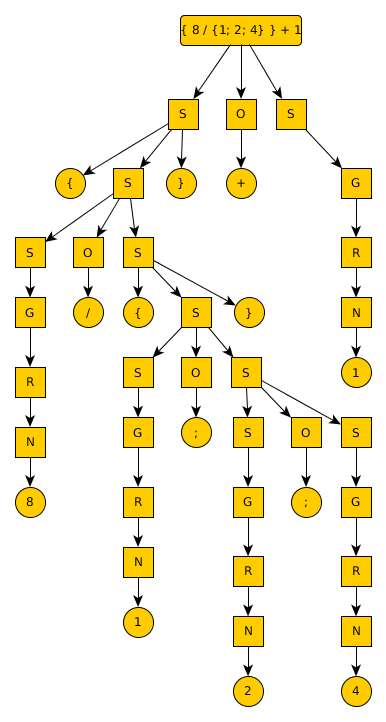
\includegraphics[scale=0.7]{arbolDerivacion2.png}}   

\centerline{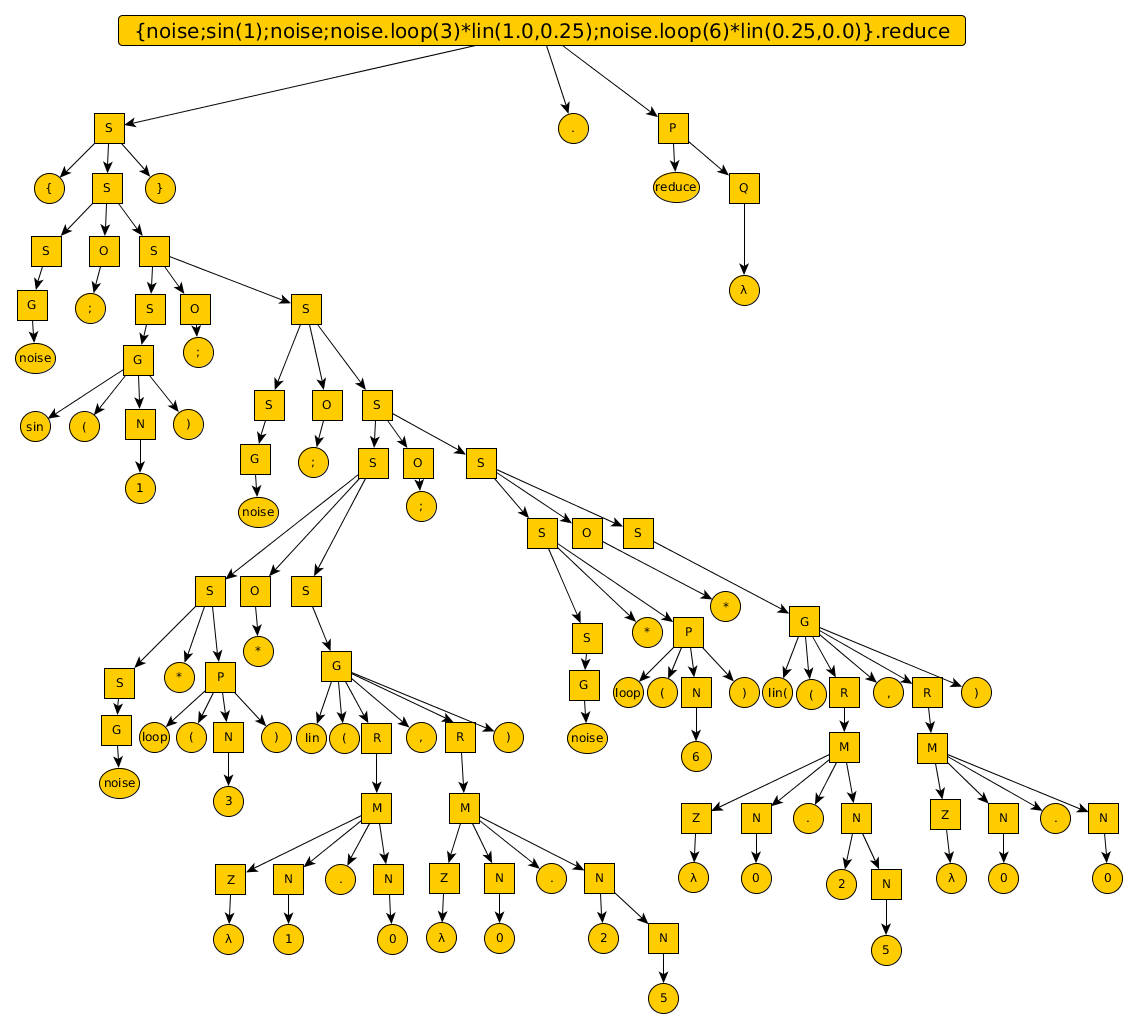
\includegraphics[scale=0.5]{arbolDerivacion.png}}   


\end{document} %Terminé!
